% Chapter 5
\chapter{Implémentation, simulation et résultats}

\label{Chapter5}
Au cours de ce chapitre nous allons présenter l'implémentation et le test de notre système dans un réseau SDN simulé. On commence par voir l'environnement de travail, les outils de simulation utilisés, pour passer ainsi à la phase des tests, qui est divisée en deux: premièrement nous allons tester notre modèle de clustering sur un jeu de données pour calculer les différentes métriques de performances citées dans la section \ref{evaluation}. L'autre partie des tests concernera notre système de détection, où nous allons définir plusieurs scénarios d'attaque et de flux normaux, pour voir son comportement et est-ce qu'il est capable d'attribuer chaque flux au bon cluster. 


\section{Environnement de travail}
Cette partie décrit l'environnement dans lequel notre solution sera déployée en présentant le contrôleur SDN choisi et l'outil de simulation du réseau utilisé.

\subsection{Contrôleur SDN}
Parmi les différents contrôleurs SDN qui existent nous avons opté pour travailler avec \textbf{Ryu}[\cite{4}] vu la simplicité d'utilisation qui offre, en plus il est basé sur \textit{Python} et supporte la majorité des versions d’OpenFlow.\\

\noindent Ryu est un contrôleur de réseau défini par logiciel (SDN) conçu pour augmenter l’agilité du réseau en le rendant facile à gérer et adapte la façon dont le trafic est traité. Il fournit des composants logiciels, avec des interfaces de programme d'applications (API) bien définies, qui rendent facile pour les développeurs de créer de nouvelles applications de gestion et de contrôle du réseau. Cette approche par composants aide les organisations à personnaliser leur déploiement pour répondre à leurs besoins spécifiques; les développeurs peuvent rapidement et facilement modifier les composants existants ou mettre en œuvre leurs propres pour s’assurer que le réseau sous-jacent peut répondre aux demandes changeantes de leurs applications.\\

\noindent Pour télécharger et installer Ryu sur une machine UBUNTU:
\begin{verbatim}
% git clone git://github.com/faucetsdn/ryu.git
% cd ryu
% pip install .
\end{verbatim}


\subsection{Simulation du réseau SDN}
Afin de pouvoir déployer notre système, nous devon simuler un réseau SDN réel avec tous ces équipements, contrôleurs SDN, commutateurs, hôtes, liens physiques. Ceci est possible à l'aide d'un émulateur réseau. Il en existe beaucoup d'émulateurs réseau, celui qui nous convient dans notre travail est \textit{Mininet}[\cite{28}].

\subsubsection{Mininet}
Mininet est un émulateur de réseau qui crée un réseau d’hôtes virtuel, de commutateurs, de contrôleurs et de liens. Les hôtes Mininet exécutent le système \textit{Linux} standard, ce qui donne la possibilité d'exécuter des programmes \textit{python} au niveau des hôtes. Les commutateurs Mininet prennent en charge Openflow pour un routage personnalisé hautement flexible.

\noindent Mininet est vaguement recommandé car:\\
\begin{itemize}
\item[-] Est rapide, démarrer un réseau simple ne prend que quelques secondes.\\
\item[-] Vous pouvez créer des topologies personnalisées : un commutateur unique, de plus grandes topologies du type Internet, un centre de données, ou toute autre chose.\\
\item[-] Vous pouvez personnaliser le transfert de paquets : les commutateurs de Mininet sont programmables à l’aide du protocole Openflow.\\
\item[-] Comprend une interface de lines de commande \textbf{CLI} pour le débogage ou l’exécution de tests sur réseau.\\
\end{itemize}

\noindent Pour installer mininet sur une machine UBUNTU:
\begin{verbatim}
% sudo apt install mininet
\end{verbatim}
Ou bien: 
\begin{verbatim}
% git clone git://github.com/mininet/mininet
% mininet/util/install.sh
\end{verbatim}

\subsubsection{Simulation d'un simple réseau SDN}
Ci-dessous un exemple sur comment lancer la simulation d'un simple réseau SDN avec un contrôleur, un switch OpenFlow et deux hôtes.\\

\noindent 1- Lancer le contôleur Ryu:
\begin{verbatim}
% ryu-manager ryu_controller.py 
\end{verbatim}
2- Créer la topologie avec mininet:
\begin{verbatim}
% sudo mn --controller remote --topo single,2 --switch ovs --mac
\end{verbatim}

\begin{tabular}{m {13cm}}
\hline
\textbf{\textit{Terminal}} - topologie créée par mininet\\
\hline
\begin{verbatim}
*** Creating network
*** Adding controller
Connecting to remote controller at 127.0.0.1:6653
*** Adding hosts:
h1 h2 
*** Adding switches:
s1 
*** Adding links:
(h1, s1) (h2, s1) 
*** Configuring hosts
h1 h2 
*** Starting controller
c0 
*** Starting 1 switches
s1 ...
*** Starting CLI:
mininet> 
\end{verbatim}\\
\hline
\end{tabular}

\section{Langage et Librairies utilisées}

\subsection{Python}
Python est un langage de programmation très puissant et adaptable à tout type d’utilisation grâce à ces bibliothèques spécialisées, utilisé particulièrement comme un langage de script. Il est trop utilisé dans la programmation réseau et spécialement dans les réseaux SDN.

\subsection{Scikit-learn}
Scikit-learn est une bibliothèque libre Python destinée à l'apprentissage automatique. Elle est développée par de nombreux contributeurs2 notamment dans le monde académique par des instituts français d'enseignement supérieur et de recherche comme Inria3. Elle comprend notamment des fonctions pour estimer des forêts aléatoires, des régressions logistiques, des algorithmes de classification, et les machines à vecteurs de support. Elle est conçue pour s'harmoniser avec d'autres bibliothèques libres Python, notamment NumPy et SciPy.[\cite{29}] 

\subsection{Pandas}
Pandas est une bibliothèque écrite pour le langage de programmation Python permettant la manipulation et l'analyse des données. Elle propose en particulier des structures de données et des opérations de manipulation de tableaux numériques et de séries temporelles. Les principales structures de données sont les séries (pour stocker des données selon une dimension - grandeur en fonction d'un index), les DataFrames (pour stocker des données selon 2 dimensions - lignes et colonnes), les Panels (pour représenter des données selon 3 dimensions, les Panels4D ou les DataFrames avec des index hiérarchiques aussi nommés MultiIndex (pour représenter des données selon plus de 3 dimensions). [\cite{30}]

\subsection{Argus}
Argus[\cite{31}] est le premier système de flux réseau, développé par Carter Bullard au début des années 1980 à Georgia Tech. La technologie de flux réseau est devenue un élément essentiel de la cybersécurité moderne et Argus est utilisé dans certains des réseaux les plus importants du monde. Le système Argus tente de résoudre un grand nombre de problèmes liés aux données de flux réseau : échelle, performance, applicabilité, confidentialité et utilité.\\

\section{Réalisation du module F-Clustering}
Rappellons que ce module est composé d'un modèle intelligent qui utilise une approche de clustering pout la détection des attaques. Dans la section \ref{F-Clustering}, nous avons décrit les étapes à suivre pour construire notre modèle de clustering qui sont accomplies à l'aide des deux scripts pythons, "Preprocessor.py" et "Cluster.Py".
\begin{algorithm}[H]
\begin{verbatim}

1- def cleanDataFrame(df):
2-  df.drop('Infinit', 'NaN')
3-  df.drop_duplicates()
4-  df.format_types()
5-  return df

6- def selectAttributs(df):
7-  return df[['Protocol', 'Flow Duration', 'Total Fwd Packets',
     'Total Backward Packets', 'Total Length of Fwd Packets',	
     'Total Length of Bwd Packets', 'Flow Bytes/s', 'Flow Packets/s', 
     'Fwd Packets/s', 'Bwd Packets/s', 'Label']]
	
   # preprocess the data frame
8- def preprocessor (df): 
9-  df = cleanDataFrame(df) #Data laundry
10- df = selectAtrributs(df) #select necessary attributs 
11- df = balanceDataFrame(df) 
12- df = scaleDataFrame(df)
13- return df

#end
\end{verbatim}
\caption{Preprocessor.py}
\end{algorithm}

\begin{algorithm}[H]
\begin{verbatim}

1- from Preprocessor.py import preprocessor 
2- from sklearn.cluster import KMeans

4- df = read_csv('TFTP.csv')

5- newDF = preprocessor(df)

6- centers = calculateCenters(newDF) #returns 2 elements array

7- F_Clustering = KMeans(n_clusters=2, init=centers).fit(newDF) 

\end{verbatim}
\caption{Cluster.py}
\end{algorithm}

\section{Évaluation et test des performances}
\label{tests}
Dans cette partie, nous allons entamer la dernière étape du processus KDD qui est l'évaluation du modèle. Comme jeu de test nous avons sélectionné le dataset « TFTP » qui contient 1.315.348 flux étiquetés (attaque et bénini). Nous avons comparé les différents résultats obtenus par notre modèle de clustering avec les données initiales du dataset pour calculer les mesures de performances du modèle.\\

\noindent Les résultats des tests de performance étaient les suivants: 

\begin{table}[H]
	\begin{center}
		\begin{tabular}{  | m{2.5cm} | m{2.5cm} | m{2.5cm} || m{2cm} | }
			\hline
			  & Attaques & Bénins & Total\\
			\hline
			Attaques & 657674 & 0 & 657674\\
			\hline
			Bénins & 8887 & 648787 & 657674\\
			\hline
		\end{tabular}
		\caption{Matrice de confusion}
	\end{center}
	\label{table:re}
\end{table}

\begin{table}[H]
	\begin{center}
		\begin{tabular}{  | c | c | c | c | c | }
			\hline
			\rowcolor[rgb]{0.85,0.85,0.85}
			 Exactitude & Précision & Rappel & F1-Measure & Taux de fausses alertes\\
			\hline
			99.3\% & 98.6\% & 100\% & 99.3\% & 1.3\%\\
			\hline
		\end{tabular}
		\caption{Mesures de performance }
	\end{center}
	\label{table:F_Clustering_Evaluation}
\end{table}

Nous remarquons que les résultats sont très satisfaisants. L'élément-clé qui nous a permis d'avoir tels résultats est le prétraitement du dataset, plus spécialement l'opération de normalisation et l'opération balancement. Pour montrer leur impact sur les performances du modèle nous allons faire une petite expérience, où nous allons annuler une opération de prétraitement à la fois, soit la normalisation, soit le balancement et calculer ensuite les mesures de performance du modèle.\\

\noindent Les résultats obtenus sont dans le tableau \ref{table:compare} et la figure \ref{fig:histogramme};
\begin{table}[h]
	\begin{center}
		\begin{tabular}{  | c | c | c | c | }
			\hline
			 Opération(s) effecutée(s) & Exactitude & Rappel & F1-Measure \\
			\hline
			\hline
			Aucune & 25.4\% & 24.4\% & 39.2\% \\
			\hline
			Normalisation seulement & 29.6\% & 27.6\% & 43.2\% \\
			\hline
			Balancement seulement & 71.5\% & 43.8\% & 60.6\% \\
			\hline
			\rowcolor[rgb]{0.9,0.70,0.70}
			Balancement + Normalisation & 99.3\% & 100\% & 99.3\% \\
			\hline
		\end{tabular}
		\caption{Impact des prétraitements sur les performances}
		\label{table:compare}
	\end{center}	
\end{table}

\begin{figure}[H]
\centering
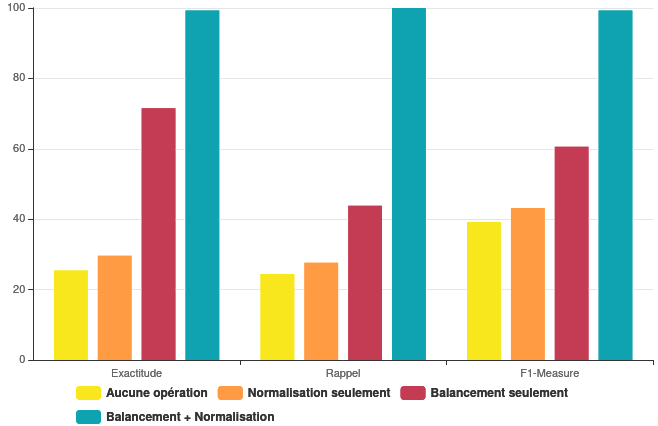
\includegraphics[width=0.95\textwidth]{Figures/performances}
\decoRule
\caption{Comparaison entre les résultats obtenus selon l'opération de prétraitement effectuée}
\label{fig:histogramme}
\end{figure} 
\newpage
En analysant l'histogramme ci-dessus on voit clairement la différence si on applique juste une seule opération de prétraitement à la fois, ou bien les deux opérations combinées. En choisissant la bonne méthode de normalisation ainsi que celle de balancement, nous avons pu faire passer le taux d'exactitude de notre modèle de \textbf{25.4\%} à \textbf{99.3\%}. Le choix des méthodes était selon une stratégie étudiée et une synthèse des résultats de plusieurs tests effectués sur notre dataset. Les bonnes performances d'un modèle sont toujours engendrées par un bon prétraitement des données.

\newpage
\section{Simulation}
La simulation sera faite à l'aide de Mininet(2.2) qui est installé à coté de Ryu(4.3) sur une machine UBUNTU 20.04 LTS dotée d'un processus i5-6200U et 8 Go de RAM. Le réseau que nous voulons simuler contient les éléments suivants: un contrôleur SDN, un switch Open Flow, un serveur de fichiers, un serveur d'applications, 3 hôtes (2 hôtes attaquants at un hôte victime), et essentiellement notre système détection F-DoS.
\begin{figure}[h]
\centering
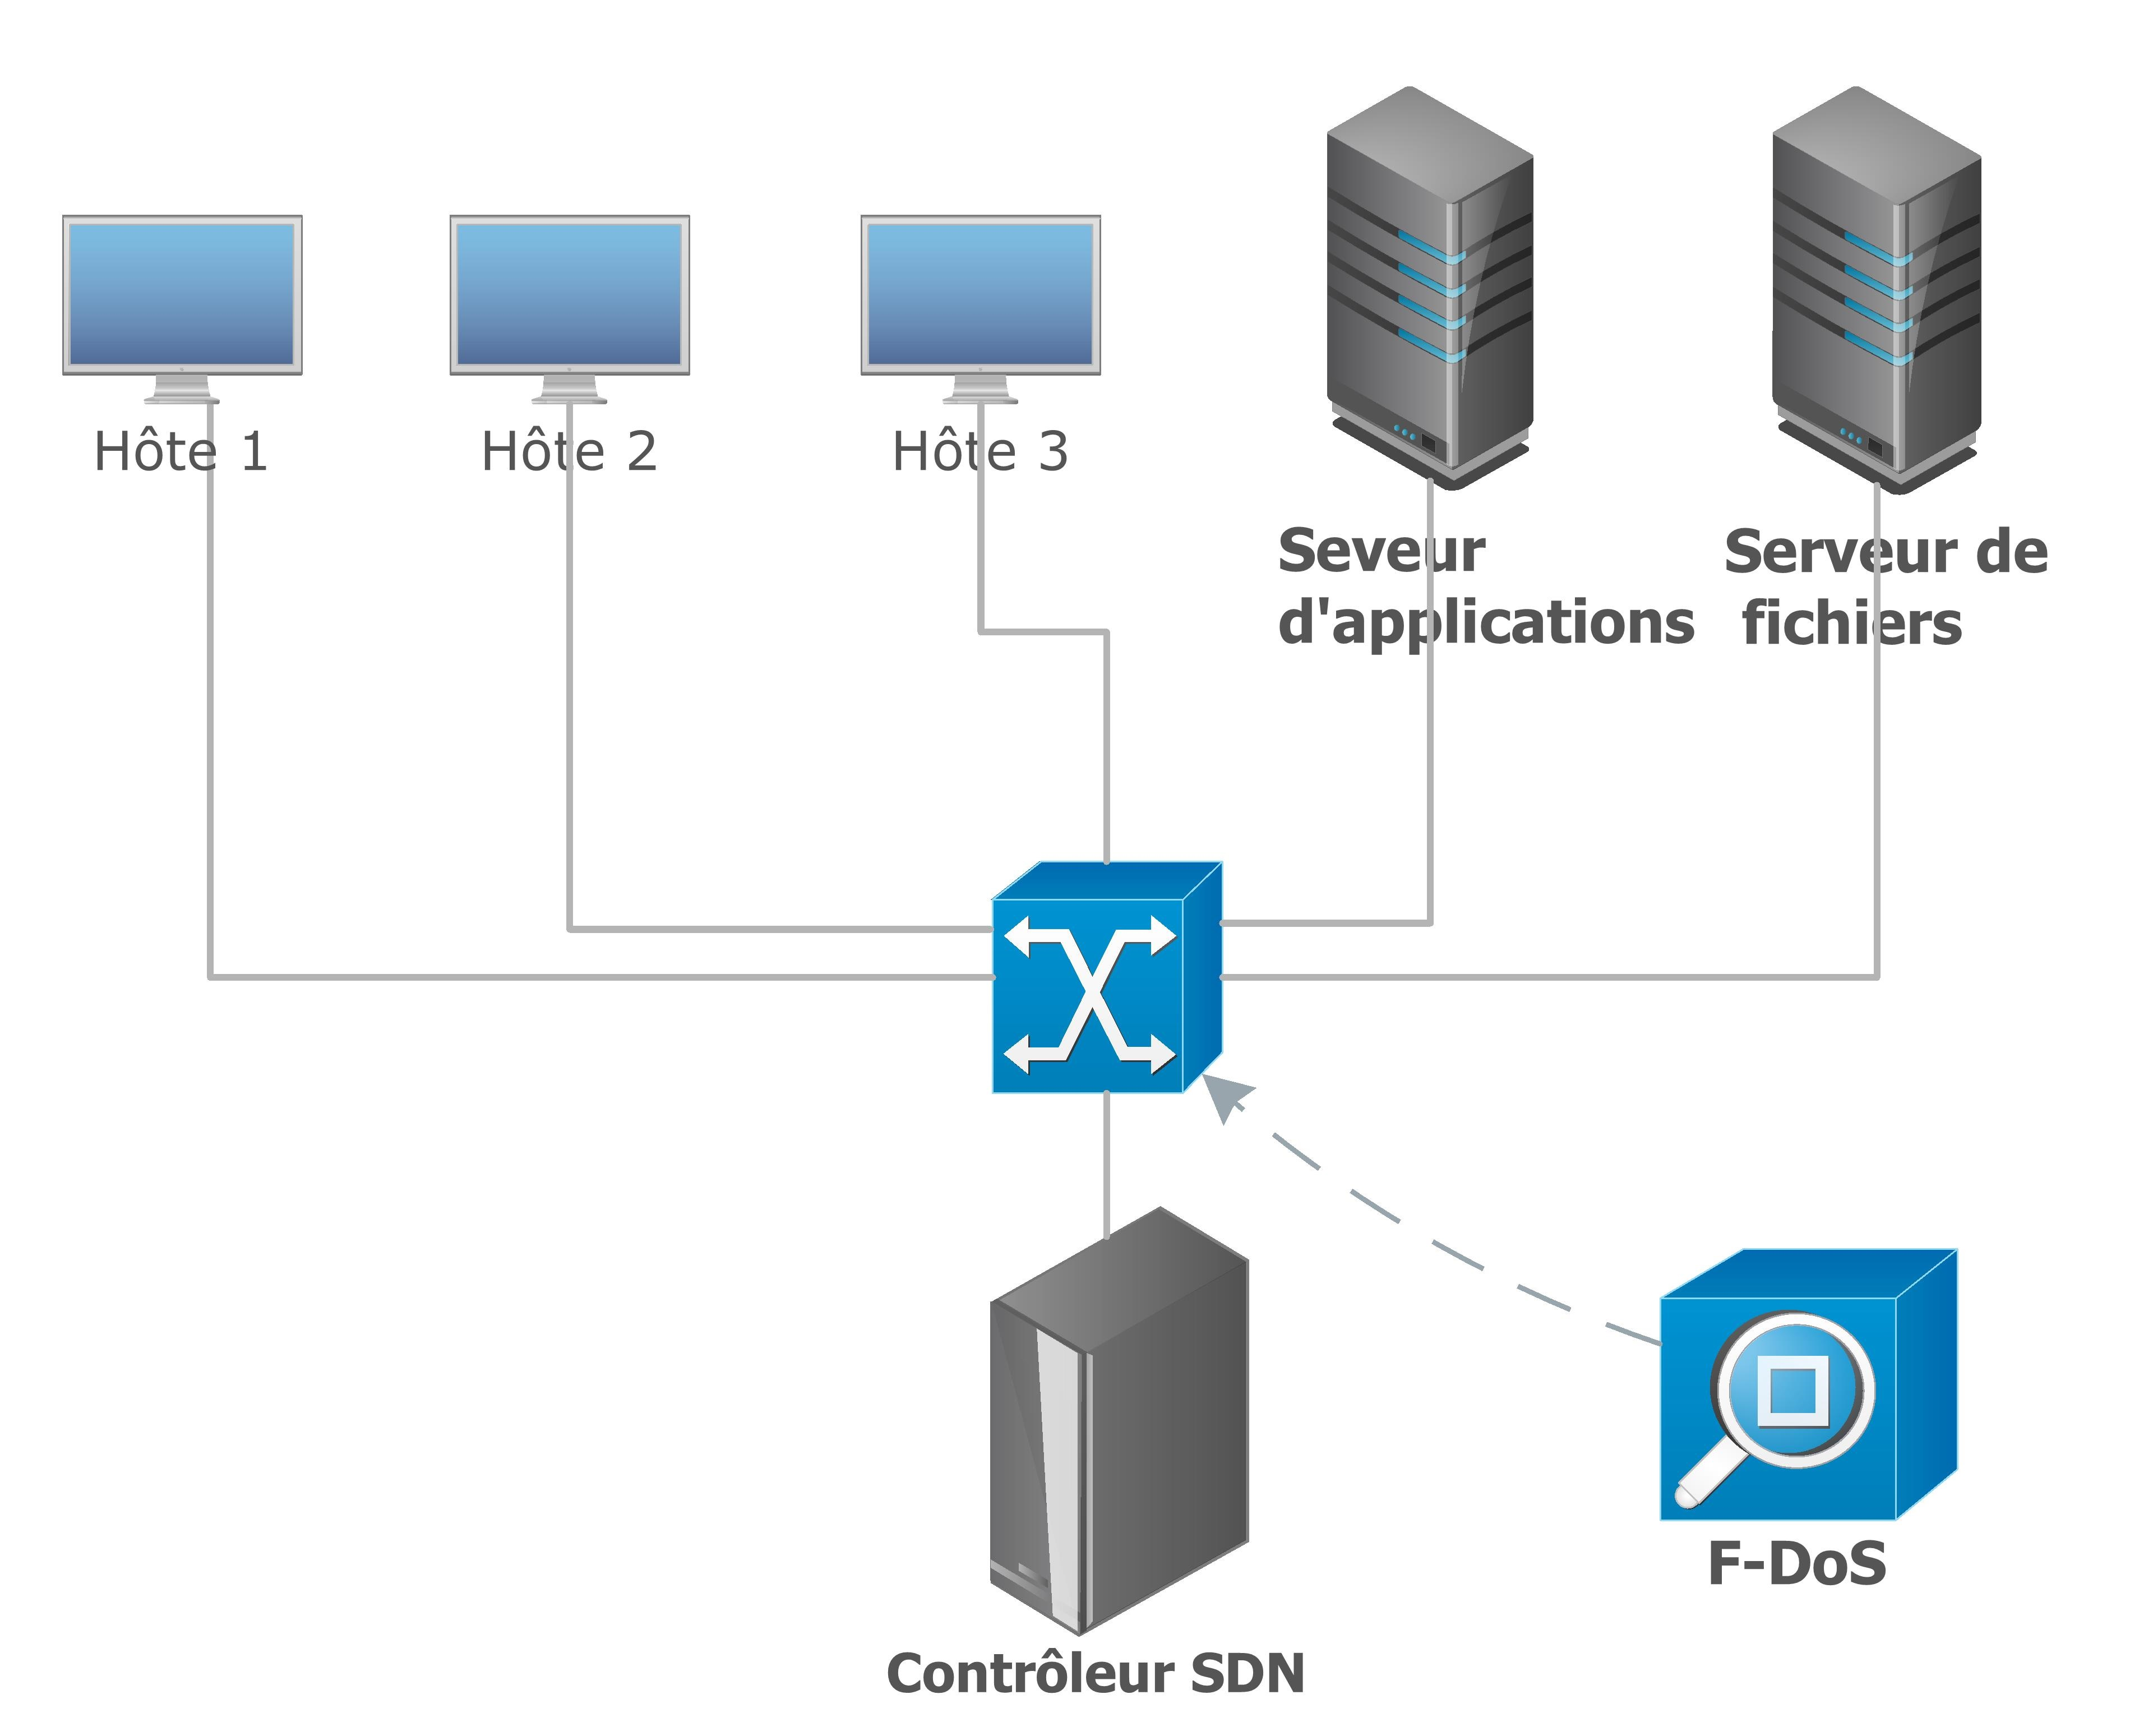
\includegraphics[width=0.8\textwidth]{Figures/simulation}
\decoRule
\caption{Architecture de notre réseau SDN}
\label{fig:architecture}
\end{figure} 

\subsection{Création de la topologie}
Sur mininet nous allons créer la topologie de notre réseau constitué d'un contrôleur SDN, un switch OpenFlow, et 6 hôtes qui jouent les rôles illustrés dans le tableau \ref{table:nodes};\\

\noindent Commande de création :
\begin{verbatim}
% sudo mn --controller remote --topo single,6 --switch ovs --mac
\end{verbatim}
Mais faut d'abord lancé le contrôleur Ryu avec:
\begin{verbatim}
% ryu-manager ryu_controller.py 
\end{verbatim}

\begin{table}[H]
\begin{center}
\begin{tabular}{  | c || m{5cm} | m{3cm} | }
\hline
\rowcolor[rgb]{0.85,0.85,0.85}
Hôte & Rôle(s) & @IP\\
\hline
\textbf{h6} & Système de détection F-DoS & 10.0.0.6\\
\hline
\textbf{h5} & Serveur d'applications & 10.0.0.5\\
\hline
\textbf{h4} & Serveur de fichiers & 10.0.0.4\\
\hline
\textbf{h3} & Hôte victime & 10.0.0.3\\
\hline
\textbf{h2} & Client de \textbf{h5} ou attaquant & 10.0.0.2\\
\hline
\textbf{h1} & Client de \textbf{h4} ou attaquant & 10.0.0.1\\
\hline
\end{tabular}
\caption{Rôle de chaque hôte dans la topologie mininet}
\label{table:nodes}
\end{center}
\end{table}

\begin{figure}[H]
\centering
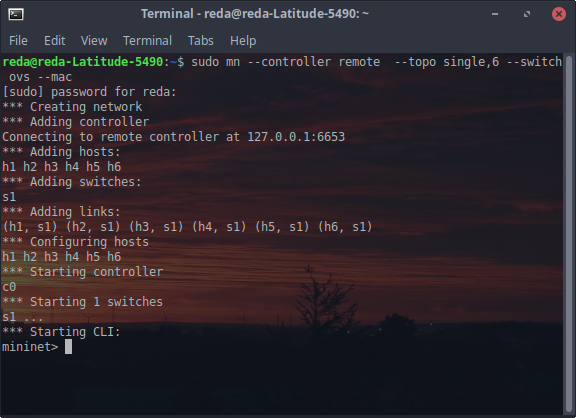
\includegraphics[width=0.7\textwidth]{Figures/simulation/mininet/start}
\decoRule
\caption{Création de la topologie sous mininet}
\label{fig:topologie}
\end{figure}

\newpage
La figure \ref{fig:topologie} indique que la topologie a été créés avec succès et la console mninet est active. On peut voir le contrôleur \textbf{c0}, le switch \textbf{s1} et les différents liens établis (h1, s1), (h2, s1), etc. L'étape suivante consiste à configurer chaque hôte de notre topologie.

\subsection{Installation des fonctions}
Jusqu'à présent les hôtes créés par mininet, ainsi que les switchs OF, n'ont que les fonctions de base définies par mininet. Donc nous devon passer par tout hôte, à l'exception de \textbf{h3}, pour installer les fonctions désignées dans le tableau \ref{table:nodes}. Sur le switch, nous allons juste activer la fonction \textit{Port-Mirroring} comme suit:

\begin{figure}[H]
\centering
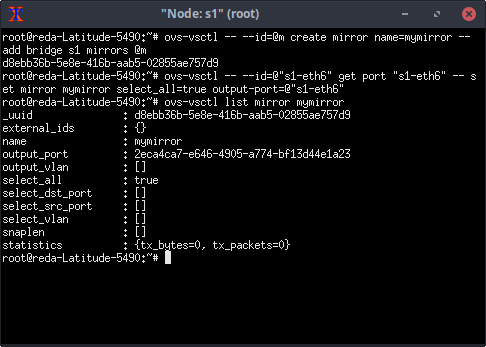
\includegraphics[width=0.8\textwidth]{Figures/simulation/mininet/switch/create_mirroring_port}
\decoRule
\caption{Activation du Port-Mirroring}
\label{fig:portMirroring}
\end{figure}

\newpage
\subsubsection{A- Installation du système F-DoS sur h6}
Sur l'hôte \textbf{h6}, nous allons installer notre système de détection. Rappelons que le module MEI du système F-DoS fait appel au client et au serveur ARGUS. Donc en premier nous allons activer le serveur ARGUS sur l'hôte h6 à l'aide de la commande suivante:
\begin{verbatim}
% sudo argus -d -i h6-eth0 -P 561 -w /captured/today.argus
\end{verbatim}
L'option \textbf{-i} : permet de spécifier l'interface d'écoute, qui est, dans notre cas, l'interface Ethernet 0 de h6.\\

\noindent Nous lançons ensuite script "IDS.py" qui va installer le client argus, ainsi que le modèle de clustering \textbf{F-Clustering}.
\begin{figure}[h]
\centering
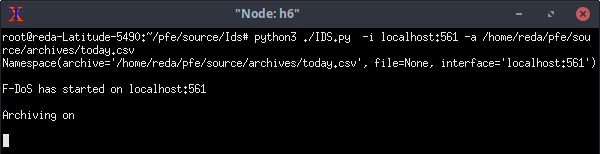
\includegraphics[width=0.9\textwidth]{Figures/simulation/mininet/IDS/start}
\decoRule
\caption{Installation du module de détection}
\label{fig:fileServer}
\end{figure}
\newpage
\subsubsection{B- Installation du serveur d'applications sur h5}
Le fonctionnement de ce serveur est basique, il se met à l'écoute des requêtes des clients, qui sont juste des messages, pour les répondre avec un message "hello". Sur l'hôte h5, le script "udpServer.py" est exécuté comme montré dans la figure \ref{fig:udpServer}.
\begin{figure}[h]
\centering
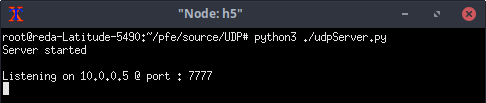
\includegraphics[width=0.9\textwidth]{Figures/simulation/mininet/UDP/server/start}
\decoRule
\caption{Installation du serveur d'applications}
\label{fig:udpServer}
\end{figure}

\subsubsection{C- Installation du serveur de fichier sur h4}
Un grand travail a été fait au niveau de cet hôte, où nous avons écrit, à partir du zéro, un script python qui lui permet de se comporter comme un serveur TFTP réel. \textbf{h4} prend en charge seulement les deux fonctions, chargement et téléchargement d'un fichier. Nous utiliserons ce serveur pour simuler le trafic TFTP qui sera capturé et analyser par notre système de détection pour l'identifier comme bénin (Téléchargement normal d'un fichier), ou bien attaque DoS. La méthode de génération des attaques réflectives va être expliquée par la suite, dans ce chapitre.
\begin{figure}[h]
\centering
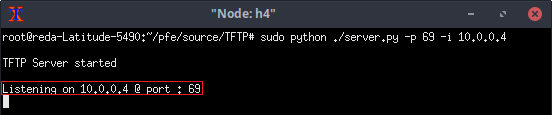
\includegraphics[width=0.9\textwidth]{Figures/simulation/mininet/TFTP/server/start}
\decoRule
\caption{Installation du seveur de fichiers}
\label{fig:udpServer}
\end{figure}

\subsubsection{D- Installation des clients}
L'hôte \textbf{h2} et l'hôte \textbf{h1} sont, respectivement, un client du serveur d'applications (client UDP) et un client du serveur de fichiers (client TFTP). Ces deux hôtes seront aussi utilisés pour lancer des attaques reflective contre ces deux serveurs, ainsi qu'une attaque du type UDP-Flooding.\\

Sur \textbf{h2} nous lançons le script "udpClient.py" qui prend comme argument le message à envoyer au serveur.
\begin{figure}[h]
\centering
\begin{subfigure}{12.5cm}
\centering
\includegraphics[width=\textwidth]{Figures/simulation/mininet/UDP/client/Benign}
\caption{Client UDP}
\end{subfigure}
\vskip 0.4cm
\begin{subfigure}{12.5cm}
\centering
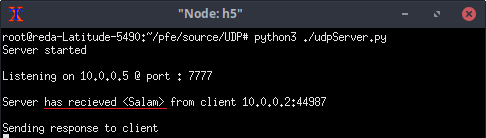
\includegraphics[width=\textwidth]{Figures/simulation/mininet/UDP/server/benign_request}
\caption{Serveur d'applications}
\end{subfigure}
\vskip 0.3cm
\decoRule
\caption{Établissement de connexion entre le client et le serveur d'applications}
\label{fig:c/s_UDP}
\end{figure}
\newpage
D'après la figure \ref{fig:c/s_UDP}, on peut voir qu'une connexion entre le seveur d'applications (@10.0.0.5) et le client (@10.0.0.2) a été établi sur le port 7777. Le client a envoyé le message \textit{"Salam"}. Le serveur lui a répondu par le message \textit{"Hello Client from Server"}. \\
Ce transfert de message a fait générer un trafic UDP qui a été capturé, en temps réel, par notre système de détection et l'a classé ce flux comme bénin, qui est bien le cas. 
\begin{figure}[h]
\centering
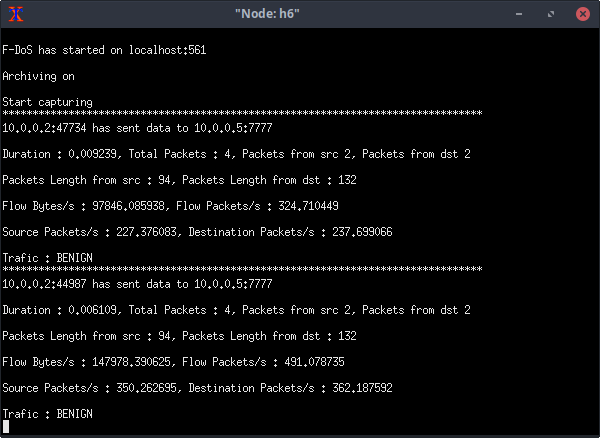
\includegraphics[width=0.85\textwidth]{Figures/simulation/mininet/IDS/benign_udp}
\decoRule
\caption{Capture et analyse du trafic UDP}
\label{fig:udpTraffic}
\end{figure}
\paragraph{}
Nous passons à l'hôte \textbf{h1}. Le script "client.py" établit une connexion avec le serveur de fichier. À l'aide de la console tftp, \textbf{h1} peut exécuter des commandes,  à distance, sur le serveur de fichier. Dans notre cas nous avons lancé une requête "get" pour télécharger le fichier \textit{"hello.txt"}, comme indiqué dans la figure \ref{fig:c/s_TFTP}.

\begin{figure}[H]
\centering
\begin{subfigure}{12.5cm}
\centering
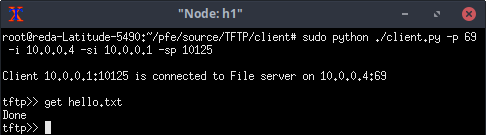
\includegraphics[width=\textwidth]{Figures/simulation/mininet/TFTP/client/benign}
\caption{Client TFTP}
\end{subfigure}
\vskip 0.4cm
\begin{subfigure}{12.5cm}
\centering
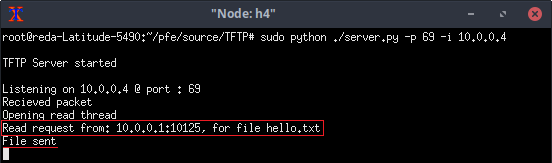
\includegraphics[width=\textwidth]{Figures/simulation/mininet/TFTP/server/benign_request}
\caption{Serveur de fichiers}
\end{subfigure}
\vskip 0.3cm
\decoRule
\caption{Établissement de connexion entre le client et le serveur de fichiers}
\label{fig:c/s_TFTP}
\end{figure}
\paragraph{}
Le transfert de fichier est réel, sur \textbf{h1} on voit le fichier téléchargé \textit{"hello.txt"}. Ce trafic de téléchargement a été aussi capturé par F-DoS et classé comme bénin, comme montré dans la figure suivante.

\begin{center}
\noindent\makebox[\textwidth]{
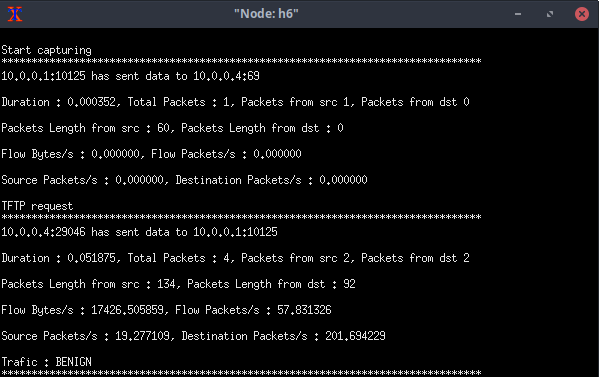
\includegraphics[width=0.82\textwidth]{Figures/simulation/mininet/IDS/benign_tftp}}%
\newline
\decoRule\\
Capture et analyse du trafic TFTP
\end{center}

\subsection{Simulation des attaques}
\subsubsection{A- Simulation de RDoS}
Rappelons que les attaques DoS reflective utilisent une adresse usurpée d'un hôte victime, pour envoyer des requêtes à un tier réflectif, qui est dans notre cas un serveur. Le serveur va répondre à la requête avec des messages réponses, mais l'hôte victime ne va pas accuser réception parce qu'il voit que ces messages ne le concernent pas et il n'a jamais lancé une telle requête, ce qui engendrera une surcharge de bande passante.\\

\noindent Pour simuler cette attaque, nous fixons comme victime l'hôte \textbf{h3} (@10.0.0.3). Au niveau de l'hôte \textbf{h1}, nous établissons une connexion avec le serveur de fichier avec l'adresse usurpée de \textbf{h3}, ensuite nous demandons le transfert du fichier \textit{"hello.txt"}.\\
\begin{figure}[H]
\centering
\begin{subfigure}{13cm}
\centering
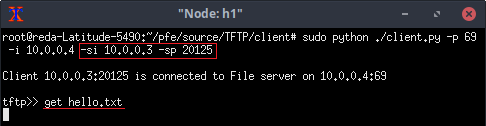
\includegraphics[width=\textwidth]{Figures/simulation/mininet/TFTP/client/attack}
\caption{Demande de téléchargement}
\end{subfigure}
\vskip 0.4cm
\begin{subfigure}{13cm}
\centering
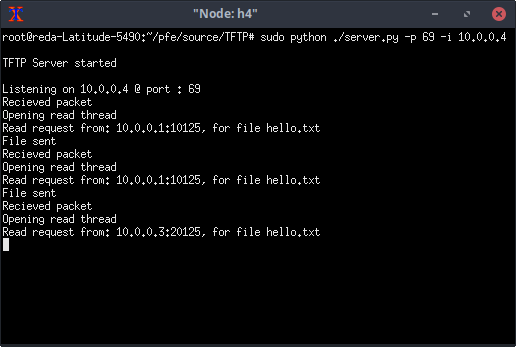
\includegraphics[width=\textwidth]{Figures/simulation/mininet/TFTP/server/attack_request}
\caption{Envoie du fichier}
\label{fig:send}
\end{subfigure}
\vskip 0.3cm
\decoRule
\caption{Simulation d'une attaque RDoS}
\label{fig:rdos_simulation}
\end{figure}
\paragraph{}
Le serveur retente plusieurs fois l'envoie du fichier à l'hôte \textbf{h3}, comme montré dans figure \ref{fig:send}, car il ne reçoit aucun accusé de la part de cet hôte pour affirmer la réception du fichier.\\

\noindent En parallel, avec l'exécution de l'attaque, qui prend un temps considérable, notre système F-DoS est toujours actif pour l'analyse du trafic. Le trafic généré par cette attaque a été capturé et belle et bien classé comme attaque (voir \ref{fig:tftpAttack}).
\begin{figure}[h]
\centering
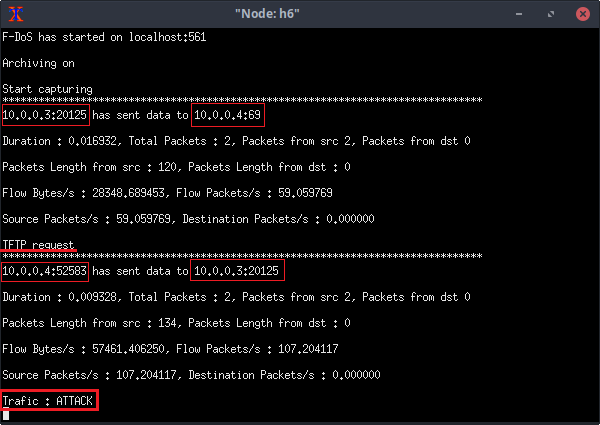
\includegraphics[width=0.87\textwidth]{Figures/simulation/mininet/IDS/attack_tftp}
\decoRule
\caption{Détection de l'attaque RDoS}
\label{fig:tftpAttack}
\end{figure}

\subsubsection{B- Simulation de UDP-Flooding}
À partir de \textbf{h2}, nous lançons une attaque du type UDP-Flooding contre \textbf{h3} (hôte victime, @10.0.0.3) à l'aide de la commande suivante :
\begin{verbatim}
% hping3 --udp --flood 10.0.0.3 -c 10 -d 400
\end{verbatim}
L'option :
\begin{itemize}
\item[\textbf{-c}]: permet de spécifier le nombre de flux.
\item[\textbf{-d}]: permet de définir la taille des données.
\end{itemize}
\begin{figure}[H]
\centering
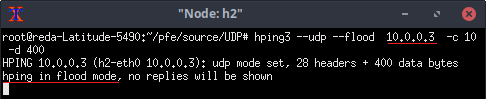
\includegraphics[width=0.9\textwidth]{Figures/simulation/mininet/UDP/attack_udp_flood}
\decoRule
\caption{Simulation d'une attaque UDP-Flooding}
\label{fig:FloodingAttackSimulation}
\end{figure}
\newpage
D'après la figure \ref{fig:FloodingAttack}, on constate que plusieurs flux ont été générés, qui est le cas d'une attaque par inondation (Flooding). F-DoS a capturé chacun de ces flux et l'a identifié comme attaque.\\

\begin{figure}[H]
\centering
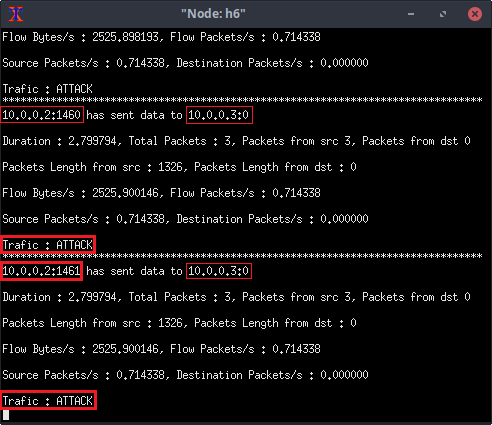
\includegraphics[width=0.9\textwidth]{Figures/simulation/mininet/IDS/attack_udp_flood}
\decoRule
\caption{Détection de l'attaque UDP-Flooding}
\label{fig:FloodingAttack}
\end{figure}

\section{Conclusion}
Au long de ce chapitre, nous avons présenté l'implémentation de notre solution de détection des attaques par déni de service dans un réseau SDN. Nous avons commencé par présenter l'environnement de travail suivi des outils utilisés pour la mise en oeuvre de notre solution. Nous avons aussi présenté la réalisation du module F-Clustering qui assure la fonction de détection des attaques en analysant les caractéristiques des flux en entrée. Pour voir l'efficacité de ce module nous l'avons mis sous le test, avec comme données de test le dataset "TFTP". Le module a montré des performances excellentes. Une précision de 98.6\% et un taux de fausses alertes de 1.3\%. Nous avons conclu, après la petite expérience faite dans la section \ref{tests} que les bonnes performances d'un modèle d'apprentissage depend, à grand part, du prétraitement des données d'apprentissage et non pas du choix de l'algorithme d'apprentissage.\\

La section la plus importante de ce chapitre était la simulation. Nous avons commencé par décrire l'architecture du réseau SDN à simuler. L'étape suivante était la création de la topologie du réseau sur Mininet suivi de l'attribution des rôles. Nous avons défini deux hôtes qui vont jouer le rôle d'un serveur, deux hôtes clients et un hôte victime. Une connexion a été établi, entre chaque serveur et son client potentiel, pour l'échange de données. À partir d'hôte, désigné comme client, une attaque RDoS a été lancé et nous avons observé le comportement de notre réseau, en particulier notre système de détection, qui a réagi en temps réel aux flux générés pour l'identifier comme attaque. Une autre du type Flooding a été simulé et notre système a été capable de la détecter.\\




 


